\chapter{Finite elements in 2D}

In Chapter~\ref{chap: FEM 1d} we considered a formally self-adjoint, linear, 
second-order differential operator~\eqref{eq: L self-adjoint}.  The 2D 
equivalent has the form
\begin{equation}\label{eq: L self-adjoint 2d}
\begin{aligned}
\mathcal{L}u&=-\nabla\cdot\bigl(a\nabla u\bigr)+cu\\
	&=-\frac{\partial}{\partial x}\biggl(a\,\frac{\partial u}{\partial x}\biggr)
	-\frac{\partial}{\partial y}\biggl(a\,\frac{\partial u}{\partial y}\biggr)
	+cu,
\end{aligned}
\end{equation}
where the coefficients $a$~and $c$ must be smooth functions of $x$~and $y$, and 
there is a constant~$a_{\min}$ such that
\[
a(x,y)\ge a_{\min}>0\quad\text{for $(x,y)\in\Omega$,}
\]
ensuring that $\mathcal{L}$ is \emph{uniformly elliptic}.  Here, as in 
Chapter~\ref{chap: finite diff 2d}, $\Omega$ is a bounded open subset 
of~$\mathbb{R}^2$ with a piecewise smooth boundary~$\Gamma=\partial\Omega$, but 
we will now suppose that
\[
\Gamma=\Gamma_{\mathrm{D}}\cup\Gamma_{\mathrm{N}},
\]
where $\Gamma_{\mathrm{D}}$~and $\Gamma_{\mathrm{N}}$ are non-overlapping, 
relatively closed subsets of~$\partial\Omega$ consisting of finitely many 
smooth curves.  (Thus, the intersection 
$\Gamma_{\mathrm{D}}\cap\Gamma_{\mathrm{N}}$ consists of finitely many
\emph{collision points}.) Our aim is to use the finite element method to compute 
numerical solutions to a \emph{mixed boundary-value problem} of the form
\begin{equation}\label{eq: self-adjoint bvp 2d}
\begin{aligned}
\mathcal{L}u&=f&&\text{in~$\Omega$,}\\
u&=g_{\mathrm{D}}&&\text{on~$\Gamma_{\mathrm{D}}$,}\\
a\,\frac{\partial u}{\partial n}&=g_{\mathrm{N}}&&
	\text{on~$\Gamma_{\mathrm{N}}$.}
\end{aligned}
\end{equation}
Here, $\partial u/\partial n$ is the derivative of~$u$ in the direction of the 
\emph{outward unit normal}~$\boldsymbol{n}$ for~$\Omega$, that is,
\[
\frac{\partial u}{\partial n}(x,y)
	=\boldsymbol{n}(x,y)\cdot\nabla u(x,y)
	\quad\text{for $(x,y)\in\partial\Omega$.}
\]
We refer to~$\Gamma_{\mathrm{D}}$~and $\Gamma_{\mathrm{N}}$ as the 
\emph{Dirichlet}~and \emph{Neumann} parts of the boundary, respectively, since 
we specify a Dirichlet boundary condition~$u=g_{\mathrm{D}}$ 
on~$\Gamma_{\mathrm{D}}$ and a Neumann boundary 
condition~$a\partial u/\partial n=g_{\mathrm{N}}$ on~$\Gamma_{\mathrm{N}}$. 

In the special case of a \emph{pure Dirichlet problem}, the Neumann part of the 
boundary is empty and so $u$ is specified on the whole of~$\Gamma$ (as 
in Chapter~\ref{chap: finite diff 2d}).  In the opposite case of a 
\emph{pure Neumann problem}, the Dirichlet part of the boundary is empty and so 
$a\,\partial u/\partial n$ is specified on the whole of~$\Gamma$.

\section{First Green identity}

Recall the \emph{divergence theorem} from vector calculus; on the right-hand 
side, the integral over~$\Gamma$ is with respect to \

\begin{theorem}\label{thm: divergence}
If the vector field $\boldsymbol{F}:\Omega\cup\Gamma\to\mathbb{R}^2$ is $C^1$, 
then
\[
\int_\Omega\nabla\cdot\boldsymbol{F}
	=\int_\Gamma\boldsymbol{F}\cdot\boldsymbol{n}.
\]
\end{theorem}

Written out more explicitly, if 
\[
\boldsymbol{F}(x,y)=P(x,y)\,\boldsymbol{i}+Q(x,y)\,\boldsymbol{j}
\quad\text{and}\quad
\boldsymbol{n}=n_x\,\boldsymbol{i}+n_y\,\boldsymbol{j},
\]
then the divergence theorem says that
\[
\iint_\Omega\biggl(\frac{\partial P}{\partial x}+\frac{\partial Q}{\partial y}
	\biggr)\,dx\,dy=\int_\Gamma\bigl(P\,n_x+Q\,n_y)\,ds,
\]
where $ds$ is the element of arc length along~$\Gamma$.  We also recall the 
following vector field identity.

\begin{lemma}\label{lem: div phi F}
For a $C^1$ scalar field~$\phi$ and a $C^1$ vector field~$\boldsymbol{F}$,
\[
\nabla\cdot(\phi\boldsymbol{F})=(\nabla\phi)\cdot\boldsymbol{F}
	+\phi\,\nabla\cdot\boldsymbol{F}.
\]
\end{lemma}

Together, Theorem~\ref{thm: divergence}~and Lemma~\ref{lem: div phi F} may be 
used to prove a 2D version of~\eqref{eq: int by parts}.

\begin{theorem}[First Green Identity]\label{thm: first Green}
If $u:\Omega\cup\Gamma\to\mathbb{R}$ is $C^2$, and if 
$v:\Omega\cup\Gamma\to\mathbb{R}$ is $C^1$, then
\[
\int_\Omega(\mathcal{L}u)\,v
	=\int_\Omega\bigl(a\nabla u\cdot\nabla v+cuv\bigr)
	-\int_\Gamma a\,\frac{\partial u}{\partial n}\,v.
\]
\end{theorem}
\begin{proof}
Taking $\phi=v$~and $\boldsymbol{F}=a\nabla u$ in Lemma~\ref{lem: div phi F}, 
we have
\[
\nabla\cdot(va\nabla u)=(\nabla v)\cdot(a\nabla u)+v\nabla\cdot(a\nabla u),
\]
so
\begin{align*}
(\mathcal{L}u)v&=\bigl(-\nabla\cdot(a\nabla u)+cu\bigr)v
	=-v\nabla\cdot(a\nabla u)+cuv\\
	&=(\nabla v)\cdot(a\nabla u)-\nabla\cdot(va\nabla u)+cuv
	=\bigl(a\nabla u\cdot\nabla v+cuv)-\nabla\cdot(va\nabla u).
\end{align*}
Applying Theorem~\ref{thm: divergence} with~$\boldsymbol{F}=va\nabla u$, it 
follows that
\[
\int_\Omega(\mathcal{L}u)v=\int_\Omega\bigl(a\nabla u\cdot\nabla v+cuv\bigr)
	-\int_\Gamma\boldsymbol(va\nabla u)\cdot\boldsymbol{n},
\]
which gives the desired identity because 
$(\nabla u)\cdot\boldsymbol{n}=\partial u/\partial n$.
\end{proof}

Since 
\[
\int_\Gamma a\,\frac{\partial u}{\partial n}\,v
	=\int_{\Gamma_{\mathrm{D}}} a\,\frac{\partial u}{\partial n}\,v
	+\int_{\Gamma_{\mathrm{N}}} a\,\frac{\partial u}{\partial n}\,v,
\]
we see that if $u$ is a $C^2$ solution of~\eqref{eq: self-adjoint bvp 2d}, and 
if $v$ is $C^1$, then
\begin{equation}\label{eq: Lu=f weak 2d}
\int_\Omega\bigl(a\nabla u\cdot\nabla v+cuv\bigr)=\int_\Omega fv
	+\int_{\Gamma_{\mathrm{N}}}g_{\mathrm{N}}v
	\quad\text{provided $v=0$ on $\Gamma_{\mathrm{D}}$.}
\end{equation}
Compare this property with its 1D equivalent~\eqref{eq: Lu=f weak 1d}.

\section{Triangulation and nodal basis}\label{sec: triangulation}

\begin{figure}
\caption{A regular triangulation.}\label{fig: good Th}
\begin{center}
\includegraphics[scale=0.8]{../src/chap6/good_triangulation.pdf}
\end{center}
\end{figure}

\begin{figure}
\caption{A triangulation that fails to be regular.}\label{fig: bad Th}
\begin{center}
\includegraphics[scale=0.8]{../src/chap6/bad_triangulation.pdf}
\end{center}
\end{figure}

Assume now that $\Omega$ is a polygon.  It follows by induction on the number 
of vertices that there exists a \emph{triangulation} of~$\Omega$, that is, a 
finite set~$\mathcal{T}$ of \emph{non-overlapping} closed triangles whose 
union is the closure of~$\Omega$. A triangulation~$\mathcal{T}$ is 
\emph{regular} if the following two conditions are satisfied:
\begin{enumerate}
\item No triangle in~$\mathcal{T}$ is \emph{degenerate}, that is, 
no~$K\in\mathcal{T}$ has collinear vertices.
\item The intersection $K_1\cap K_2$ of any two distinct triangles $K_1$, 
$K_2\in\mathcal{T}$ is either empty, a common edge or a common vertex.
\end{enumerate}
For example, Figure~\ref{fig: good Th} shows a regular triangulation with 
7~vertices, or \emph{nodes}, numbered in red, and 6~triangles, or 
\emph{elements}, numbered in blue.  (The six boundary edges are 
numbered in green.) However, the triangulation in 
Figure~\ref{fig: bad Th} is not regular: the intersection of triangles 2~and 6 
is an edge of triangle~6 but is not (the whole of) an edge of triangle~2.
Vertex~7 in Figure~\ref{fig: bad Th} is said to be a \emph{hanging node}.

A simple data structure to store a triangulation consists of three arrays,
$\boldsymbol{N}$, $\boldsymbol{T}^{\mathcal{K}}$ and
$\boldsymbol{T}^{\mathcal{E}}$.  The first stores the coordinates of the
$r$th node in its $r$th column, the second stores the node numbers of the
$p$th triangle~$K_p$ in its $p$th column, and the third stores the node numbers
of the $q$th boundary edge~$E_q$ in its $q$th column.  Thus, the triangulation
in Figure~\ref{fig: good Th} may be described by
\[
\boldsymbol{N}=\begin{bmatrix}
 0&-2& 2& 2& 1&-1&-2\\
 0&-2&-2& 0& 2& 2& 0
\end{bmatrix},\qquad
\boldsymbol{T}^{\mathcal{K}}=\begin{bmatrix}
7&2&3&4&5&6\\
2&3&4&5&6&7\\
1&1&1&1&1&1
\end{bmatrix},
\]
and
\[
\boldsymbol{T}^{\mathcal{E}}=\begin{bmatrix}
7&2&3&4&5&6\\
2&3&4&5&6&7 \end{bmatrix}.
\]
We call $\boldsymbol{T}^{\mathcal{K}}$ the \emph{triangle connectivity matrix}
and call $\boldsymbol{T}^{\mathcal{E}}$ the \emph{edge connectivity matrix}.
To simplify some geometric computations, it is best to ensure that the node
numbering within each triangle proceeds counterclockwise, and that the edge
node numbering follows the induced orientation of~$\partial\Omega$. (Even with 
this restriction, there are $3$~possibilities for each column 
of~$\boldsymbol{T}$.)

Denote the maximum element diameter 
by~$h=\max_{K\in\mathcal{T}}\operatorname{diam}(K)$, and let $V_h$ denote the 
vector space consisting of those functions~$v:\Omega\cup\Gamma\to\mathbb{R}$ 
that are continuous and piecewise-linear with respect to~$\mathcal{T}$.  Thus,
if $v\in V_h$ then for each~$K\in\mathcal{T}$ there are coefficients 
$c\brak{K}_0$, $c\brak{K}_1$~and $c\brak{K}_2$ such that
\begin{equation}\label{eq: v K 1 x y}
v(x,y)=c\brak{K}_0+c\brak{K}_1x+c\brak{K}_2y
	\quad\text{for $(x,y)\in K$.}
\end{equation}
Let $\mathsf{n}\brak{K}_1$, $\mathsf{n}\brak{K}_2$, $\mathsf{n}\brak{K}_3$ 
denote the vertices of the triangle~$K$, and let $\psi\brak{K}_1$, 
$\psi\brak{K}_2$, $\psi\brak{K}_3$ denote the unique linear functions 
satisfying
\begin{equation}\label{eq: psi node triangle}
\psi\brak{K}_j(\mathsf{n}\brak{K}_i)=\delta_{jk}
	\quad\text{for $i$, $j\in\{1,2,3\}$.}
\end{equation}
In Section~\ref{sec: barycentric}, we will derive explicit representations of 
these functions.  The property~\eqref{eq: psi node triangle} implies that if 
$v\in V_h$ then
\[
v(x,y)=\sum_{i=1}^3v(\mathsf{n}\brak{K}_i)\psi\brak{K}_i(x,y)
	\quad\text{for $(x,y)\in K$,}
\]
showing that $v$ is uniquely determined by its values at the nodes 
of~$\mathcal{T}$.

\begin{figure}
\caption{A piecewise-linear ``tent function'', equal to~$1$ at one node, and 
$0$ at all other nodes.}\label{fig: tent func}
\begin{center}
\includegraphics[scale=0.6]{../src/chap6/tent_func.pdf}
\end{center}
\end{figure}

If $K=K_p$ then we write $\mathsf{n}_i\brak{p}=\mathsf{n}_i\brak{K_p}$ and
$\psi\brak{p}_i=\psi\brak{K_p}_i$.  Given a global enumeration $\mathsf{n}_1$,
$\mathsf{n}_2$, \dots, $\mathsf{n}_M$ of the nodes of~$\mathcal{T}$, as
determined by the triangle connectivity
matrix~$\boldsymbol{T}^{\mathcal{K}}=[t^{\mathcal{K}}_{ip}]$, we have
\[
\mathsf{n}_r=\mathsf{n}\brak{p}_i\quad\text{iff}\quad r=t^{\mathcal{K}}_{ip}.
\]
Likewise, let $\mathsf{n}^{[q]}_j$ denote the $j$th vertex ($j=1$, $2$) of
the $q$th edge~$E_q$.  The entries of the $2\times Q$ edge connectivity
matrix~$\boldsymbol{T}^{\mathcal{E}}=[t^{\mathcal{E}}_{jq}]$ are such that
\[
\mathsf{n}_r=\mathsf{n}^{[q]}_j \quad\text{iff}\quad r=t^{\mathcal{E}}_{jq}.
\]
In the natural way, we define the linear shape functions for the edge~$E_q$ by
\[
\psi^{[q]}_1(x,y)=1-\xi\quad\text{and}\quad
\psi^{[q]}_2(x,y)=\xi\quad\text{if}\quad
(x,y)=(1-\xi)\mathsf{n}^{[q]}_1+\xi\mathsf{n}^{[q]}_2,
\]
so that
\begin{equation}\label{eq: psi node edge}
\psi^{[q]}_j(\mathsf{n}^{[q]}_k)=\delta_{jk}\quad\text{for $j$, $k\in\{1,2\}$,}.
\end{equation}

For~$1\le r\le M$, we define the nodal basis function~$\chi_r\in V_h$ by
requiring
\begin{equation}\label{eq: chi 2d}
\chi_r(\mathsf{n}_s)=\delta_{rs}\quad\text{for $r$, $s\in\{1, 2, \dots, M\}$.}
\end{equation}
Figure~\ref{fig: tent func} shows an example of such a ``tent function''.  
The properties \eqref{eq: psi node triangle}~and \eqref{eq: chi 2d} imply that
\begin{equation}\label{eq: chi psi}
\chi_r(x,y)=\psi\brak{p}_i(x,y)
\quad\text{for $(x,y)\in K_p$ if $r=t^{\mathcal{K}}_{ip}$.}
\end{equation}
and likewise by~\eqref{eq: psi node edge},
\[
\chi_r(x,y)=\psi^{[q]}_j(x,y)
\quad\text{for $(x,y)\in E_q$ if $r=t^{\mathcal{E}}_{jq}$.}
\]

If $v\in V_h$, then
\[
v(x,y)=\sum_{r=1}^M v(\mathsf{n}_r)\chi_r(x,y)
	\quad\text{for $(x,y)\in\Omega\cup\Gamma$,}
\]
and we call $\{\chi_1,\chi_2,\ldots,\chi_M\}$ the \emph{nodal basis} for~$V_h$
(Exercise~\ref{ex: nodal basis}).

\section{Finite element method}

Suppose that a regular triangulation~$\mathcal{T}$ is \emph{aligned} with 
the decomposition $\Gamma=\Gamma_{\mathrm{D}}\cup\Gamma_{\mathrm{N}}$ of the 
boundary of~$\Omega$.  This assumption means that $\Gamma_{\mathrm{D}}$ 
is a union of edges of triangles in~$\mathcal{T}$ (in which 
case, the same must be true of~$\Gamma_{\mathrm{N}}$).  The vertices lying on 
the Dirichlet boundary~$\Gamma_{\mathrm{D}}$ are called the \emph{fixed nodes}, 
because the values of the solution~$u$ are fixed at these points.  The 
remaining vertices are called the \emph{free nodes}; these belong 
to~$\Omega\cup\Gamma_{\mathrm{N}}$, but note that the collision points, where
$\Gamma_{\mathrm{D}}$~and $\Gamma_{\mathrm{N}}$ meet, are among the fixed nodes.

We let
\begin{align*}
M&=\text{number of vertices in the triangulation},\\
P&=\text{number of triangles in $\mathcal{K}$,}\\
Q&=\text{number of edge elements on $\partial\Omega$,}
\end{align*}
and denote the sets of vertices (nodes), triangles (elements) and boundary edges
by
\begin{align*}
\mathcal{N}&=\{\mathsf{n}_1,\mathsf{n}_2,\ldots,\mathsf{n}_M\},\\
\mathcal{K}&=\{K_1,K_2,\ldots,K_P\},\\
\mathcal{E}&=\{E_1,E_2,\ldots,E_Q\}.
\end{align*}
The sets of \emph{free nodes} and \emph{fixed nodes} are denoted by
\[
\mathcal{N}\free
        =\{\,\mathsf{n}\in\mathcal{N}:\mathsf{n}\not\in\GammaD\,\}
\quad\text{and}\quad
\mathcal{N}\fix
        =\{\,\mathsf{n}\in\mathcal{N}:\mathsf{n}\in\GammaD\,\}.
\]
The sets of \emph{Dirichlet edges} and \emph{Neumann edges} are denoted by
\[
\EdgeD=\{\,E\in\mathcal{E}:E\subseteq\GammaD\,\}
\quad\text{and}\quad
\EdgeN=\{\,E\in\mathcal{E}:E\subseteq\GammaN\,\}.
\]
We then have the disjoint unions
\[
\mathcal{N}=\mathcal{N}\free\cup\mathcal{N}\fix
\quad\text{and}\quad
\mathcal{E}=\EdgeD\cup\EdgeN.
\]
The nodes are numbered so that the free ones precede the fixed ones:
\[
\mathcal{N}\free=\{\,\mathsf{n}_m:1\le m\le M\free\,\}
\]
and
\[
\mathcal{N}\fix=\{\,\mathsf{n}_m:M\free+1\le m\le M\,\}.
\]
Likewise, for the edges,
\[
\EdgeN=\{\,E_q:1\le q\le Q\free\,\}
\quad\text{and}\quad
\EdgeD=\{\,E_q:Q\free+1\le q\le Q\,\}.
\]

Let $g_{\mathrm{D},h}:\Gamma_{\mathrm{D}}\to\mathbb{R}$ be a piecewise-linear 
approximation to~$g_{\mathrm{D}}$.  An obvious choice is the interpolant, so
that
\[
g_{\mathrm{D},h}(\mathsf{n}_r)=g(\mathsf{n}_r)
    \quad\text{for $M\free+1\le r\le M$.}
\]
We define the trial set
\[
S_h=\{\,v\in V_h:\text{$v=g_{\mathrm{D},h}$ on $\Gamma_{\mathrm{D}}$}\,\}
\]
and the test space
\[
T_h=\{\,v\in V_h:\text{$v=0$ on $\Gamma_{\mathrm{D}}$}\,\}.
\]
Recalling \eqref{eq: Lu=f weak 2d}, the finite element 
solution~$u_h\in S_h$ is then defined by requiring that
\begin{equation}\label{eq: FEM 2d}
\int_\Omega\bigl(a\nabla u_h\cdot\nabla v+cu_hv\bigr)=\int_\Omega fv
	+\int_{\Gamma_{\mathrm{N}}}g_{\mathrm{N}}v
	\quad\text{for all $v\in T_h$.}
\end{equation}

We expand the finite element solution in the nodal basis, and enforce the 
Dirichlet boundary condition to obtain the representation
\begin{equation}\label{eq: uh U 2d}
u_h(x,y)=\sum_{s=1}^MU_s\chi_s(x,y)=\sum_{s=1}^{M\free}U_s\chi_s(x,y)
    +\sum_{s=M\free+1}^M g_{D,h}(\mathsf{n}_s)\chi_s(x,y).
\end{equation}
Since $\{\chi_1,\chi_2,\ldots,\chi_{M\free}\}$ is a basis for the trial 
space~$T_h$, the requirement~\eqref{eq: FEM 2d} is equivalent to
\begin{equation}\label{eq: FEM 2d alt}
\int_\Omega\bigl(a\nabla u_h\cdot\nabla\chi_r+cu_h\chi_r\bigr)
    =\int_\Omega f\chi_r
    -\int_{\Gamma_{\mathrm{N}}}g_{\mathrm{N}}\chi_r
    \quad\text{for $1\le r\le M\free$,}
\end{equation}
and so, after inserting the representation~\eqref{eq: uh U 2d}, we obtain an 
$M\free\times M\free$~linear system
\begin{equation}\label{eq: FEM 2D linear system}
\sum_{s=1}^{M\free}\bigl(a_{rs}+c_{rs}\bigr)U_s
    =f_r+g_{\mathrm{N},r}-\sum_{s=M\free+1}^M(a_{rs}+c_{rs})g_{\mathrm{D},s}
    \quad\text{for $1\le r\le M\free$,}
\end{equation}
where
\[
a_{rs}=\int_\Omega a\nabla\chi_s\cdot\nabla\chi_r,\qquad
c_{rs}=\int_\Omega c\chi_s\chi_r,\qquad
f_r=\int_\Omega f\chi_r,\qquad
g_{\mathrm{N},r}=\int_{\Gamma_{\mathrm{N}}}g_{\mathrm{N}}\chi_r,
\]
and $g_{\mathrm{D},s}=g_{\mathrm{D},h}(\boldsymbol{n}_s)$. Let 
\[
\boldsymbol{U}=[U_s]_{s=1}^M
    =\begin{bmatrix}\boldsymbol{U}\free\\ \boldsymbol{U}\fix \end{bmatrix}
\quad\text{where}\quad
\boldsymbol{U}\free=\begin{bmatrix}U_1\\ U_2\\ \vdots\\ U_{M\free}\end{bmatrix}
\quad\text{and}\quad
\boldsymbol{U}\fix=\begin{bmatrix}U_{M\free+1}\\ U_{M\free+2}\\ \vdots\\ U_M
\end{bmatrix},
\]
and 
\[
\boldsymbol{A}=[a_{rs}]_{\substack{1\le r\le M\free\\ 1\le s\le M}}
=[\,\boldsymbol{A}\free\quad\boldsymbol{A}\fix\,]
\]
where
\[
\boldsymbol{A}\free=\begin{bmatrix}
a_{11}&\cdots&a_{1M\free}\\
\vdots&\ddots&\vdots\\
a_{M\free1}&\cdots&a_{M\free M\free}
\end{bmatrix}
\quad\text{and}\quad
\boldsymbol{A}\fix=\begin{bmatrix}
a_{1,M\free+1}&\cdots&a_{1M}\\
\vdots&\ddots&\vdots\\
a_{M\free,M\free+1}&\cdots&a_{M\free,M}
\end{bmatrix}.
\]
Similarly, $\boldsymbol{C}=[\boldsymbol{C}\free\quad\boldsymbol{C}\fix]$, and 
we can write the linear system~\eqref{eq: FEM 2D linear system} as
\begin{equation}\label{eq: 2D FEM linear system}
\bigl(\boldsymbol{A}\free+\boldsymbol{C}\free\bigr)\boldsymbol{U}\free
    =\boldsymbol{f}+\boldsymbol{g}_{\mathrm{N}}
-\bigl(\boldsymbol{A}\fix+\boldsymbol{C}\fix\bigr)\boldsymbol{g}_{\mathrm{D}}
\quad\text{and}\quad
\boldsymbol{U}\fix=\boldsymbol{g}_{\mathrm{D}},
\end{equation}
with
\[
\boldsymbol{f}=\begin{bmatrix}f_1\\ f_2\\ \vdots\\ f_{M\free}\end{bmatrix},
\qquad
\boldsymbol{g}_{\mathrm{N}}=\begin{bmatrix}
g_{\mathrm{N},1}\\ g_{\mathrm{N},2}\\ \vdots\\ 
g_{\mathrm{N},M\free}\end{bmatrix},
\qquad
\boldsymbol{g}_{\mathrm{D}}=\begin{bmatrix}
g_{\mathrm{D},M\free+1}]\\ g_{\mathrm{D},M\free+2}]\\ \vdots\\
g_{\mathrm{D},M}] 
\end{bmatrix}.
\]

\section{Barycentric coordinates and element matrices}\label{sec: barycentric}

Consider a triangle~$K$ with vertices $\boldsymbol{a}_1$, 
$\boldsymbol{a}_2$~and $\boldsymbol{a}_3$.  The \emph{barycentric coordinates} 
$(\xi_1,\xi_2,\xi_3)$ of a point~$\boldsymbol{x}$ with respect to~$K$ are 
defined by the relations
\[
\boldsymbol{x}=\xi_1\boldsymbol{a}_1+\xi_2\boldsymbol{a}_2
    +\xi_3\boldsymbol{a}_3
    \quad\text{and}\quad
\xi_1+\xi_2+\xi_3=1.    
\]
Thus, $\boldsymbol{a}_1$, $\boldsymbol{a}_2$, $\boldsymbol{a}_3$ have
barycentric coordinates $(1,0,0)$, $(0,1,0)$, $(0,0,1)$, respectively. We will 
see below that each~$\xi_p$ is a linear function of~$\boldsymbol{x}$, so 
\begin{equation}\label{eq: xi psi}
\xi_p=\psi_p\brak{K}(\boldsymbol{x})
    \quad\text{for $1\le p\le 3$,}
\end{equation}
where the $\psi_p\brak{K}$ are the linear linear shape functions introduced in 
Section~\ref{sec: triangulation}.  Thus, a level set of any
barycentric coordinate is a straight line, as illustrated 
in~\ref{fig: barycentric}.

\begin{figure}
\caption{Level sets of the barycentric coordinates 
$(\xi_1,\xi_2,\xi_3)$, and the centroid~$\boldsymbol{c}$.}
\label{fig: barycentric}
\begin{center}
\includegraphics[scale=0.75]{../src/chap6/barycentric.pdf}
\end{center}
\end{figure}

Let $\boldsymbol{B}$ denote the inverse transpose 
(Exercise~\ref{ex: inv transpose}) of the matrix with columns 
$\boldsymbol{a}_1-\boldsymbol{a}_3$~and $\boldsymbol{a}_1-\boldsymbol{a}_3$, 
that is,
\[
\boldsymbol{B}=[\,(\boldsymbol{a}_1-\boldsymbol{a}_3)\quad
    (\boldsymbol{a}_1-\boldsymbol{a}_3)\,]^{-T},
\]
and write
\begin{equation}\label{eq: bp vector def}
\boldsymbol{B}=[\,\boldsymbol{b}_1\quad\boldsymbol{b}_2\,]
\quad\text{with}\quad\boldsymbol{b}_3=-(\boldsymbol{b}_1+\boldsymbol{b}_2).
\end{equation}
The \emph{centroid} of~$K$ is the point
\[
\boldsymbol{c}=\tfrac13\boldsymbol{a}_1+\tfrac13\boldsymbol{a}_2
+\tfrac13\boldsymbol{a}_3
\]
with barycentric coordinates~$(\tfrac13,\tfrac13,\tfrac13)$. The barycentric 
coordinates of a given point~$\boldsymbol{x}$ can be computed as follows.

\begin{theorem}\label{thm: barycentric}
With the notation above,
\[
\xi_j=\tfrac13+\boldsymbol{b}_j\cdot(\boldsymbol{x}-\boldsymbol{c})
\quad\text{for $j\in\{1,2,3\}$.}
\]
\end{theorem}
\begin{proof}
Since $\xi_1+\xi_2+\xi_3=1$ we can express $\boldsymbol{x}$ in terms of 
$\xi_1$~and $\xi_2$ only,
\[
\boldsymbol{x}=\xi_1\boldsymbol{a}_1+\xi_2\boldsymbol{a}_2
    +(1-\xi_1-\xi_2)\boldsymbol{a}_3
    =\boldsymbol{a}_3+\xi_1(\boldsymbol{a}_1-\boldsymbol{a}_3)
    +\xi_2(\boldsymbol{a}_2-\boldsymbol{a}_3).
\]
Thus,
\[
\boldsymbol{x}-\boldsymbol{a}_3
=[\,(\boldsymbol{a}_1-\boldsymbol{a}_3)\quad
    (\boldsymbol{a}_2-\boldsymbol{a}_3\,]
\begin{bmatrix}\xi_1\\ \xi_2 \end{bmatrix}
=B^{-T}\begin{bmatrix}\xi_1\\ \xi_2 \end{bmatrix}
\]
and so
\[
\begin{bmatrix}\xi_1\\ \xi_2 \end{bmatrix}=B^T(\boldsymbol{x}-\boldsymbol{a}_3)
=\begin{bmatrix}\boldsymbol{b}_1^T\\ \boldsymbol{b}_2^T\end{bmatrix}
    (\boldsymbol{x}-\boldsymbol{a}_3)
=\begin{bmatrix}\boldsymbol{b}_1\cdot(\boldsymbol{x}-\boldsymbol{a}_3)\\
\boldsymbol{b}_2\cdot(\boldsymbol{x}-\boldsymbol{a}_3)\end{bmatrix},
\]
that is,
\[
\xi_1=\boldsymbol{b}_1\cdot(\boldsymbol{x}-\boldsymbol{a}_3)
\quad\text{and}\quad
\xi_2=\boldsymbol{b}_2\cdot(\boldsymbol{x}-\boldsymbol{a}_3),
\]
Since $\boldsymbol{a}_1$, $\boldsymbol{a}_2$, $\boldsymbol{a}_3$ have
barycentric coordinates $(1,0,0)$, $(0,1,0)$, $(0,0,1)$, respectively,
\[
\boldsymbol{b}_1\cdot(\boldsymbol{a}_1-\boldsymbol{a}_3)
=1=\boldsymbol{b}_2\cdot(\boldsymbol{a}_2-\boldsymbol{a}_3)
\]
whereas
\[
\boldsymbol{b}_1\cdot(\boldsymbol{a}_2-\boldsymbol{a}_3)
=0=\boldsymbol{b}_2\cdot(\boldsymbol{a}_1-\boldsymbol{a}_3),
\]
so, for $j\in\{1,2\}$,
\[
\boldsymbol{b}_j\cdot(\boldsymbol{c}-\boldsymbol{a}_3)
    =\boldsymbol{b}_j\cdot(
\tfrac13\boldsymbol{a}_1+\tfrac13\boldsymbol{a}_2+\tfrac13\boldsymbol{a}_3
    -\boldsymbol{a}_3)
    =\tfrac13\boldsymbol{b}_j\cdot(\boldsymbol{a}_1-\boldsymbol{a}_3)
    +\tfrac13\boldsymbol{b}_j\cdot(\boldsymbol{a}_2-\boldsymbol{a}_3)
    =\tfrac13
\]
and hence
\[
\xi_j=\boldsymbol{b}_j\cdot(
    \boldsymbol{x}-\boldsymbol{c}+\boldsymbol{c}-\boldsymbol{a}_3)
    =\boldsymbol{b}_j\cdot(\boldsymbol{x}-\boldsymbol{c})+\tfrac13.
\]
Finally,
\[
\xi_3=1-\xi_2-\xi_3=(1-\tfrac13-\tfrac13)
    -(\boldsymbol{b}_1+\boldsymbol{b}_2)\cdot
    (\boldsymbol{x}-\boldsymbol{a}_3)
    =\tfrac13+\boldsymbol{b}_3\cdot(\boldsymbol{x}-\boldsymbol{a}_3).
\]
\end{proof}

We define the triangular reference element
\[
K_{\mathrm{ref}}=\{\,(\xi_1,\xi_2):
    \text{$0\le\xi_1\le1$ and $0\le\xi_2\le 1-\xi_1$}\,\}
\]
with reference nodes $\boldsymbol{n}_p=\boldsymbol{a}_p$ for~$1\le p\le 3$,
and observe that the affine transformation $K_{\mathrm{ref}}\to K$ defined by
\[
(\xi_1,\xi_2)\mapsto\boldsymbol{x}(\xi_1,\xi_2)=\boldsymbol{a}_3
    +\xi_1(\boldsymbol{a}_1-\boldsymbol{a}_3)
    +\xi_2(\boldsymbol{a}_2-\boldsymbol{a}_3)
\]
is one-one and onto, with Jacobian determinant
\[
\frac{\partial(x_1,x_2)}{\xi_1,\xi_2})
    =\det[\,(\boldsymbol{a}_1-\boldsymbol{a}_3)\quad
            (\boldsymbol{a}_2-\boldsymbol{a}_3)\,].
\]
Since $\bigl|\det[\,(\boldsymbol{a}_1-\boldsymbol{a}_3)\quad
(\boldsymbol{a}_2-\boldsymbol{a}_3)\,]\bigr|$ equals the area of the 
parallelogram spanned by the vectors $\boldsymbol{a}_1-\boldsymbol{a}_3$~and 
$\boldsymbol{a}_2-\boldsymbol{a}_3$, which in turns equals $2\mathrm{area}(K)$, 
it follows that
\begin{equation}\label{eq: int K f}
\int_Kf=2\,\mathrm{area}(K)\int_0^1\int_0^{1-\xi_1}
    f\bigl(\boldsymbol{x}(\xi_1,\xi_2)\bigr)\,d\xi_2\,d\xi_1.
\end{equation}
The formula in the next theorem allows us to compute $\int_Kf$ for any 
polynomial~$f$.

\begin{theorem}\label{thm: int xi}
For all non-negative integers $n_1$, $n_2$, $n_3$,
\[
\int_K\xi_1^{n_1}\xi_2^{n_2}\xi_3^{n_3}=2\,\mathrm{area}(K)\,
    \frac{n_1!\,n_2!\,n_3!}{(n_1+n_2+n_3+2)!}.
\]
\end{theorem}
\begin{proof}
By~\eqref{eq: int K f},
\begin{align*}
\int_K\xi_1^{n_1}\xi_2^{n_2}\xi_3^{n_3}&=2\,\mathrm{area}(K)
    \int_0^1\int_0^{1-\xi_1}\xi_1^{n_1}\xi_2^{n_2}(1-\xi_1-\xi_2)^{n_3}
        \,d\xi_2\,d\xi_1\\
    &=2\,\mathrm{area}(K)
    \int_0^1\xi_1^{n_1}\int_0^{1-\xi_1}\xi_2^{n_2}(1-\xi_1-\xi_2)^{n_3}
        \,d\xi_2\,d\xi_1.
\end{align*}
Integrating by parts $m$~times, we see that for any~$a>0$,
\begin{align*}
\int_0^a\,\frac{\xi^n}{n!}\,\frac{(a-\xi)^m}{m!}\,d\xi
&=\int_0^a\,\frac{\xi^{n+1}}{(n+1)!}\,\frac{(a-\xi)^{m-1}}{(m-1)!}\,d\xi\\
&=\cdots
=\int_0^a\,\frac{\xi^{n+m}}{(n+m)!}\,d\xi=\frac{a^{n+m+1}}{(n+m+1)!},
\end{align*}
so
\begin{multline*}
\int_0^1\xi_1^{n_1}\int_0^{1-\xi_1}\xi_2^{n_2}(1-\xi_1-\xi_2)^{n_3}
        \,d\xi_2\,d\xi_1
    =n_2!\,n_3!\int_0^1\xi_1^{n_1}\int_0^{1-\xi_1}
    \frac{\xi_2^{n_2}}{n_2!}\,\frac{(1-\xi_1-\xi_2)^{n_3}}{n_3!}
        \,d\xi_1\,d\xi_1\\
    =n_1!\,n_2!\,n_3!\int_0^1\frac{\xi_1^{n_1}}{n_1!}\,
        \frac{(1-\xi_1)^{n_2+n_3+1}}{(n_2+n_3+1)!}\,d\xi_1
    =\frac{n_1!\,n_2!\,n_3!}{(n_1+n_2+n_3+2)!},
\end{multline*}
giving the desired formula.
\end{proof}

\begin{figure}
\caption{The vectors $\boldsymbol{b}_1$, $\boldsymbol{b}_2$~and 
$\boldsymbol{b}_3$ defined in~\eqref{eq: bp vector def}.}\label{fig: b vectors}
\begin{center}
\includegraphics[scale=0.8]{../src/chap6/b_vectors-crop.pdf}
\end{center}
\end{figure}

Recalling \eqref{eq: xi psi}~and Theorem~\ref{thm: barycentric}, the linear 
shape functions are given by
\[
\psi_j(\boldsymbol{x})=\xi_j
    =\tfrac13+\boldsymbol{b}_j\cdot(\boldsymbol{x}-\boldsymbol{a}_j)
    \quad\text{for $j\in\{1,2,3\}$,}
\]
and so
\[
\nabla\psi_j=\boldsymbol{b}_j\quad\text{for $j\in\{1,2,3\}$.}
\]
Thus, $\boldsymbol{b}_j$ is orthogonal to the level sets of~$\psi_j$ and in 
particular to the side of~$K$ opposite~$\boldsymbol{a}_j$, as shown in 
Figure~\ref{fig: b vectors}.

Using the same approach as in the 1D case in 
Section~\ref{sec: matrix assembly 1d}, we will assemble the 
$M\times(M+R)$ global stiffness 
matrix~$\boldsymbol{A}=[\,\boldsymbol{A}'\quad\boldsymbol{A}'']$ from 
the $3\times3$ element stiffness matrices
\[
\boldsymbol{A}\brak{K}=\bigl[a\brak{K}_{ij}\bigr]_{i,j=1}^3
\quad\text{where}\quad
a\brak{K}_{ij}=\int_Ka\nabla\psi_j\brak{K}\cdot\nabla\psi\brak{K}_i.
\]
Likewise, the $M\times(M+R)$ global mass 
matrix~$\boldsymbol{C}=[\,\boldsymbol{C}'\quad\boldsymbol{C}'']$ will be 
assembled from the $3\times3$ element mass matrices,
\[
\boldsymbol{C}\brak{K}=\bigl[c\brak{K}_{ij}\bigr]_{i,j=1}^3
\quad\text{where}\quad
c\brak{K}_{ij}=\int_Kc\psi_j\brak{K}\psi\brak{K}_i.
\]
Explicitly, the entries of the element stiffness matrix are
\[
a\brak{K}_{ij}=\boldsymbol{b}_j\cdot\boldsymbol{b}_i\int_K a
    =\boldsymbol{b}_j\cdot\boldsymbol{b}_i\int_0^1\int_0^{1-\xi_1}
        a\bigl(\boldsymbol{x}(\xi_1,\xi_2)\bigr)\,d\xi_2\,d\xi_1,
\]
and those of the element mass matrix are
\[
c\brak{K}_{ij}=\int_Kc\xi_j\xi_i=\int_0^1\int_0^{1-\xi_1}
        c\bigl(\boldsymbol{x}(\xi_1,\xi_2)\bigr)\xi_j\xi_i\,d\xi_2\,d\xi_1,
\]
remembering that $\xi_3=1-\xi_1-\xi_2$.
In particular, if $a(\boldsymbol{x})=1$~and $c(\boldsymbol{x})=1$, then
Theorem~\ref{thm: int xi} shows that 
\begin{equation}\label{eq: AK CK}
\newcommand{\bb}{\boldsymbol{b}}
\boldsymbol{A}\brak{K}=\mathrm{area}(K)\begin{bmatrix}
\bb_1\cdot\bb_1&\bb_2\cdot\bb_1&\bb_3\cdot\bb_1\\
\bb_1\cdot\bb_2&\bb_2\cdot\bb_2&\bb_3\cdot\bb_2\\
\bb_1\cdot\bb_3&\bb_2\cdot\bb_3&\bb_3\cdot\bb_3
\end{bmatrix}
\quad\text{and}\quad
\boldsymbol{C}\brak{K}=\frac{\mathrm{area}(K)}{12}\begin{bmatrix}
2&1&1\\ 1&2&1\\ 1&1&2 \end{bmatrix}.
\end{equation}

The 3-dimensional element load vector is defined by
\[
\boldsymbol{f}\brak{K}=[f\brak{K}_i]_{i=1}^3
\quad\text{where}\quad
f\brak{K}_i=\int_K f\psi\brak{K}_i
	=\int_0^1\int_0^{1-\xi_1}f\bigl(\boldsymbol{x}(\xi_1,\xi_2)\bigr)\xi_i
	\,d\xi_2 \,d\xi_1.
\]
Similarly, the 2-dimensional Neumann load vector is defined by
\[
\boldsymbol{g}^{[E]}_{\mathrm{N}}=[g^{[E]}_{\mathrm{N},j}]_{j=1}^2
\quad\text{where}\quad
g^{[E]}_{\mathrm{N},j}=\int_E g_{\mathrm{N}}\psi^{[E]}_j,
\]
that is,
\[
g^{[E]}_{\mathrm{N},1}
    =\int_0^1g_{\mathrm{N}}\bigl(\boldsymbol{x}(\xi)\bigr)(1-\xi)\,d\xi
\quad\text{and}\quad
g^{[E]}_{\mathrm{N},2}
    =\int_0^1g_{\mathrm{N}}\bigl(\boldsymbol{x}(\xi)\bigr)\xi\,d\xi
\]
where $\boldsymbol{x}(\xi)=(1-\xi)\mathsf{n}^{[E]}_1+\xi\mathsf{n}^{[E]}_2$
parameterises~$E$.


\section{Assembling the linear system}

The process of assembling the global linear
system~\eqref{eq: 2D FEM linear system} works the same way as in 1D.  We
define the index sets
\[
\mathcal{J}^{\mathcal{K}}_r=\{\,(p,i):\mathsf{n}_r=\mathsf{n}\brak{p}_i\,\}
    =\{\,(p,i):r=t^{\mathcal{K}}_{ip}\,\}
\]
and
\[
\mathcal{J}^{\mathcal{E}}_r=\{\,(q,j):\mathsf{n}_r=\mathsf{n}^{[q]}_j\,\}
    =\{\,(p,j):r=t^{\mathcal{E}}_{jq}\,\}
\]
and find that the components of the load vector are
\[
f_r=\int_\Omega f\chi_r=\sum_{p=1}^P\int_{K_p}f\chi_r
    =\sum_{(p,i)\in\mathcal{J}^{\mathcal{K}}_r}\int_{K_p}f\psi\brak{p}_i
    =\sum_{(p,i)\in\mathcal{J}^{\mathcal{K}}_r}f\brak{p}_i,
\]
resulting in \cref{alg: assemble f piecewise linear 2D}. Similarly for the
Neumann load vector,
\[
g_{\mathrm{N},r}=\int_{\GammaN}g_{\mathrm{N}}\chi_r
    =\sum_{q=1}^{Q\free}\int_{E_q}g_{\mathrm{N}}\chi_r
    =\sum_{(q,j)\in\mathcal{J}^{\mathcal{E}}_r}
        \int_{E_q}g_{\mathrm{N}}\psi^{[q]}_j
    =\sum_{(q,j)\in\mathcal{J}^{\mathcal{E}}_r}g_{\mathrm{N},j}^{[q]},
\]
resulting in \cref{alg: assemble gN piecewise linear 2D}.  Note that
the usual convention applies regarding an empty sum: $g_{\mathrm{N},r}=0$ if
$\mathcal{J}^{\mathcal{E}}_r=\emptyset$, which will be the case, for example,
whenever $\mathsf{n}_r$ is an interior node.

\begin{algorithm}
\caption{Assemble the load vector $\boldsymbol{f}$ for a piecewise linear FEM in
2D.}\label{alg: assemble f piecewise linear 2D}
\begin{algorithmic}
\State $\boldsymbol{f}=\boldsymbol{0}\in\mathbb{R}^{M\free}$
\For{$p=1:P$}
    \State Compute $\boldsymbol{f}\brak{p}$
    \For{$i=1:3$}
        \State $r=t^{\mathcal{K}}_{pi}$
                                  \Comment{$\mathsf{n}_r=\mathsf{n}\brak{p}_i$}
        \If{$r\le M\free$}
            \State $f_r\gets f_r+f\brak{p}_i$
        \EndIf
    \EndFor
\EndFor
\end{algorithmic}
\end{algorithm}

\begin{algorithm}
\caption{Assemble the Neumann load vector $\boldsymbol{g}_{\mathrm{N}}$ for a
piecewise linear FEM in 2D.}
\label{alg: assemble gN piecewise linear 2D}
\begin{algorithmic}
\State $\boldsymbol{g}_{\mathrm{N}}=\boldsymbol{0}\in\mathbb{R}^{M\free}$
\For{$q=1:Q$}
    \State Compute $\boldsymbol{g}_{\mathrm{N}}^{[q]}$
    \For{$j=1:2$}
        \State $r=t^{\mathcal{E}}_{pj}$
                                     \Comment{$\mathsf{n}_r=\mathsf{n}{[q]}_j$}
        \If{$r\le M\free$}
            \State $g_{\mathrm{N},r}\gets
                    q_{\mathrm{N},r}+g^{[q]}_{\mathrm{N},j}$
        \EndIf
    \EndFor
\EndFor
\end{algorithmic}
\end{algorithm}


Turning the stiffness matrix, we define as in 1D
\[
\mathcal{J}^{\mathcal{K}}_{rs}=\{\,(p,i,j):
    \text{$\mathsf{n}_r=\mathsf{n}\brak{p}_{ip}$ and
    $\mathsf{n}_s=\mathsf{n}\brak{p}_{jp}$}\,\}
\]
and find that
\begin{align*}
a_{rs}&=\int_\Omega a\nabla\chi_s\cdot\nabla\chi_r
    =\sum_{p=1}^P\int_{K_p}a\nabla\chi_s\cdot\nabla\chi_r\\
    &=\sum_{(p,i,j)\in\mathcal{J}^{\mathcal{K}}_{rs}}
    \int_{K_p}a\nabla\psi\brak{p}_j\cdot\nabla\psi\brak{p}_i
    =\sum_{(p,i,j)\in\mathcal{J}^{\mathcal{K}}_{rs}}a\brak{p}_{ij},
\end{align*}
resulting in \cref{alg: assemble A piecewise linear 2D}. Similarly, for the mass
matrix
\[
c_{rs}=\sum_{(p,i,j)\in\mathcal{J}^{\mathcal{K}}_{rs}}c\brak{p}_{ij}.
\]
In practice, we would not store $\boldsymbol{A}$ and $\boldsymbol{C}$ as dense
$M\free\times M$ arrays, but would instead a sparse matrix format such as CSC.

\begin{algorithm}
\caption{Assemble the stiffness matrix $\boldsymbol{A}$ for a piecewise linear
FEM in 2D.}
\label{alg: assemble A piecewise linear 2D}
\begin{algorithmic}
\State $\boldsymbol{A}=\boldsymbol{0}\in\mathbb{R}^{M\free\times M}$
\For{$p=1:P$}
    \State Compute $\boldsymbol{A}\brak{p}$
    \For{$j=1:3$}
        \State $r=t^{\mathcal{K}}_{jp}$
        \If{$r\le M\free$}
            \For{$k=1:3$}
                \State $s=t^{\mathcal{K}}_{kp}$
                \State $a_{rs}\gets a_{rs}+a\brak{p}_{jk}$
            \EndFor
        \EndIf
    \EndFor
\EndFor
\end{algorithmic}
\end{algorithm}



\section{Quadratic elements}

\begin{figure}
\caption{The midpoint $\boldsymbol{m}_j$ of the side opposite to the 
vertex~$\boldsymbol{a}_j$ for $j\in\{1,2,3\}$.}
\label{fig: midpoints}
\begin{center}
\includegraphics[scale=0.75]{../src/chap6/midpoints.pdf}
\end{center}
\end{figure}

\begin{figure}
\caption{Quadratic shape functions}
\label{fig: quad shape funcs}
\hfil
\includegraphics[scale=0.8]{../src/chap6/quad_shape_funcs/psi1-crop.pdf}
\hfil
\includegraphics[scale=0.8]{../src/chap6/quad_shape_funcs/psi2-crop.pdf}
\hfil
\includegraphics[scale=0.8]{../src/chap6/quad_shape_funcs/psi3-crop.pdf}
\hfil
\\[2\jot]
\includegraphics[scale=0.8]{../src/chap6/quad_shape_funcs/psi4-crop.pdf}
\hfil
\includegraphics[scale=0.8]{../src/chap6/quad_shape_funcs/psi5-crop.pdf}
\hfil
\includegraphics[scale=0.8]{../src/chap6/quad_shape_funcs/psi6-crop.pdf}
\hfil
\end{figure}


A general quadratic polynomial in two variables $x_1$~and $x_2$ has the form
\[
v(x_1,x_2)=a_{00}+a_{10}x_1+a_{01}x_2+a_{20}x_1^2+a_{11}x_1x_2+a_{02}x_2^2.
\]
Thus, the space of all such polynomials has dimension~$6$ and we therefore 
require $6$ nodes in our triangular element~$K$. For $j\in\{1,2,3\}$, let 
$\boldsymbol{m}_j$ denote the midpoint of the side of the triangle~$K$ opposite 
the vertex~$\boldsymbol{a}_j$, as illustrated in
\cref{fig: midpoints}.  The barycentric coordinates of $\boldsymbol{m}_1$, 
$\boldsymbol{m}_2$, $\boldsymbol{m}_3$ are then $(0,\tfrac12,\tfrac12)$,
$(\tfrac12,0,\tfrac12)$, $(\tfrac12,\tfrac12,0)$, respectively.  We then define 
our 6~nodes in the element~$K$ by
\[
\boldsymbol{n}\brak{K}_1=\boldsymbol{a}_1,\quad
\boldsymbol{n}\brak{K}_2=\boldsymbol{a}_2,\quad
\boldsymbol{n}\brak{K}_3=\boldsymbol{a}_3,\quad
\boldsymbol{n}\brak{K}_4=\boldsymbol{m}_1,\quad
\boldsymbol{n}\brak{K}_5=\boldsymbol{m}_2,\quad
\boldsymbol{n}\brak{K}_6=\boldsymbol{m}_3,
\]
and the corresponding quadratic shape functions~$\psi\brak{K}_j$ 
for~$1\le \le 6$ by requiring that
\[
\psi\brak{K}_j(\boldsymbol{n}\brak{K}_i)=\delta_{ij}
\quad\text{for $i$, $j\in\{1,2,3,4,5,6\}$.}
\]
As functions of the barycentric coordinates, we easily verify that
\[
\psi\brak{K}_1(\boldsymbol{x})=2\xi_1(\xi_1-\tfrac12),\qquad
\psi\brak{K}_2(\boldsymbol{x})=2\xi_2(\xi_2-\tfrac12),\qquad
\psi\brak{K}_3(\boldsymbol{x})=2\xi_3(\xi_3-\tfrac12),
\]
and
\[
\psi\brak{K}_4(\boldsymbol{x})=4\xi_2\xi_3,\qquad
\psi\brak{K}_5(\boldsymbol{x})=4\xi_3\xi_1,\qquad
\psi\brak{K}_6(\boldsymbol{x})=4\xi_1\xi_2.
\]
\cref{fig: quad shape funcs} plots these functions for a typical triangle.
Since $\nabla\xi_j=\boldsymbol{b}_j$, 
\[
\nabla\psi\brak{K}_j(\boldsymbol{x})=(4\xi_j-1)\boldsymbol{b}_j
\quad\text{for $1\le j\le 3$,}
\]
and
\begin{align*}
\nabla\psi\brak{K}_4(\boldsymbol{x})
    &=4(\xi_2\boldsymbol{b}_3+\xi_3\boldsymbol{b}_2),\\
\nabla\psi\brak{K}_5(\boldsymbol{x})
    &=4(\xi_3\boldsymbol{b}_1+\xi_1\boldsymbol{b}_3),\\
\nabla\psi\brak{K}_6(\boldsymbol{x})
    &=4(\xi_1\boldsymbol{b}_2+\xi_2\boldsymbol{b}_1).
\end{align*}
Using \cref{thm: int xi}



\section{Optimality property}

We assume that the coefficients are continuous on
$\overline{\Omega}=\Omega\cup\partial\Omega$, and satisfy
\[
a(x,y)\ge a_{\min}>0\quad\text{and}\quad c(x,y)\ge c_{\min}\ge0
    \quad\text{for $(x,y)\in\Omega$.}
\]
Generalising the definition of the energy inner product in 1D, we let
\[
\iprod{u,v}_{\mathcal{L}}=\int_\Omega\bigl(a\nabla u\cdot\nabla v
    +cuv\bigr)
\]
and denote the associated energy norm by
\[
\|u\|_{\mathcal{L}}=\sqrt{\iprod{u,u}_{\mathcal{L}}}.
\]
Thus,
\[
\|u\|_{\mathcal{L}}^2=\int_\Omega\bigl(a\|\nabla u\|^2+cu^2\bigr).
\]

The weak solution of the mixed boundary-value 
problem~\eqref{eq: self-adjoint bvp 2} satisfies the 
essential boundary condition~$u=g_{\mathrm{D}}$ on~$\GammaD$ together with the
property~\eqref{eq: Lu=f weak 2d} which can be written as
\[
\iprod{u,v}_{\mathcal{L}}=\iprod{f,v}+\iprod{g_{\mathrm{N}},v}_{\GammaN}
\quad\text{whenever $v=0$ on $\GammaD$.}
\]
Similarly the finite element solution~$u_h\in S_h$ satisfies~\eqref{eq: FEM 2d} 
which can be written as
\[
\iprod{u_h,v}_{\mathcal{L}}=\iprod{f,v}+\iprod{g_{\mathrm{N}},v}_{\GammaN}
\quad\text{whenever $v\in T_h$.}
\]
The Galerkin orthogonality property follows at once,
\[
\iprod{u_h-u,v}_{\mathcal{L}}=0\quad\text{for all $v\in T_h$,}
\]
and we deduce the optimality property of~$u_h$ using the same argument as in 
1D; see \cref{thm: optimality}.

\begin{theorem}\label{thm: optimality 2D}
The finite element solution~$u_h\in S_h$ of the mixed boundary-value 
problem~\eqref{eq: self-adjoint bvp 2} satisfies
\[
\|u_h-u\|_{\mathcal{L}}\le\|w-u\|_{\mathcal{L}}
	\quad\text{for all $w\in S_h$.}
\]
\end{theorem}
\begin{proof}
Let $w\in S_h$ and observe that the error~$e_h=u_h-u$ satisfies
\begin{align*}
\|e_h\|_{\mathcal{L}}^2=\iprod{e_h,e_h}_{\mathcal{L}}
	&=\iprod{e_h,u_h-u}_{\mathcal{L}}
	=\iprod{e_h,u_h-w+w-u}_{\mathcal{L}}\\
	&=\iprod{e_h,u_h-w}_{\mathcal{L}}+\iprod{e_h,w-u}_{\mathcal{L}}.
\end{align*}
Since both $u_h$ and $w$ belong to~$S_h$, 
their difference $u_h-w=g_{\mathrm{D}}-g_{\mathrm{D}}=0$ on~$\GammaD$, showing
that $u_h-w\in T_h$.  Hence, the Galerkin orthogonality 
property~\eqref{eq: energy orthog} implies
that $\iprod{e_h,u_h-w}_{\mathcal{L}}=0$ so, by the Cauchy--Schwarz inequality,
\[
\|e_h\|_{\mathcal{L}}^2=\iprod{e_h,w-u}_{\mathcal{L}}
	\le\|e_h\|_{\mathcal{L}}\|w-u\|_{\mathcal{L}},
\]
which implies the desired inequality.
\end{proof}



\begin{Exercises}

\exercise
Suppose that $\Omega=\Omega_1\cup\Gamma_{\mathrm{i}}\cup\Omega_2$ where the
\emph{interface}~$\Gamma_{\mathrm{i}}$ is a piecewise smooth curve, and that
\[
a(x,y)=\begin{cases}
a_1(x,y)&\text{for $(x,y)\in\Omega_1$,}\\
a_2(x,y)&\text{for $(x,y)\in\Omega_2$.}
\end{cases}
\]
Define corresponding partial differential operators
$\mathcal{L}_ku=-\nabla\cdot(a_k\nabla u)$ on $\Omega_k$ for~$k\in\{1,2\}$.
Suppose that
\[
\mathcal{L}_ku_k=f_k\quad\text{on $\Omega_k$ for $k\in\{1,2\}$,}
\]
and define
\[
u(x,y)=\begin{cases}
u_1(x,y)&\text{for $(x,y)\in\Omega_1$,}\\
u_2(x,y)&\text{for $(x,y)\in\Omega_2$,}
\end{cases}
\qquad\text{and}\qquad
f(x,y)=\begin{cases}
f_1(x,y)&\text{for $(x,y)\in\Omega_1$,}\\
f_2(x,y)&\text{for $(x,y)\in\Omega_2$.}
\end{cases}
\]
Under what condition(s) on $u_1$~and $u_2$ do $u$~and $f$ satisfy
\[
\int_\Omega a\nabla u\cdot\nabla v
    =\int_{\partial\Omega}a\,\frac{\partial u}{\partial n}\,v
    +\int_\Omega fv
\]
for any test function~$v$?  Hint: let $\boldsymbol{n}_{\mathrm{i}}$ denote the
unit normal along~$\Gamma_{\mathrm{i}}$, outward to~$\Omega_1$ and inward
to~$\Omega_2$.

\exercise
Derive the weak formulation of the boundary-value 
problem \eqref{eq: self-adjoint bvp 2d} if we replace the Neumann boundary
condition with the, more general, Robin boundary condition,
\[
a\,\frac{\partial u}{\partial n}+bu=g_{\mathrm{N}}
\quad\text{on $\Gamma_{\mathrm{N}}$,}
\]
for a given coefficient~$b(x)$.
\begin{ans}
The weak solution $u$ satisfies
\[
\int_\Omega(a\nabla u\cdot\nabla v+cuv)+\int_{\Gamma_{\mathrm{N}}}buv
=\int_\Omega fv+\int_{\Gamma_{\mathrm{N}}}g_{\mathrm{N}} v 
\quad\text{whenever $v=0$ on~$\Gamma_{\mathrm{D}}$,}
\]
with $u=g_{\mathrm{D}}$ on $\Gamma_{\mathrm{D}}$.
\end{ans}

\exercise
Derive the weak formulation for the elliptic eigenproblem
\[
\begin{aligned}
\mathcal{L}\phi&=\lambda b\phi&&\text{in $\Omega$},\\
\phi&=0&&\text{on $\Gamma_{\mathrm{D}}$,}\\
a\,\frac{\partial\phi}{\partial n}&=0&&\text{on $\Gamma_{\mathrm{N}}$,}
\end{aligned}
\]
where, as usual, $\mathcal{L}\phi=-\nabla\cdot(a\nabla\phi)+c\phi$.
\begin{ans}
The eigenpair $(\phi,\lambda)$ satisfies
\[
\int_\Omega(a\nabla\phi\cdot\nabla v+c\phi v)=\lambda\int_\Omega b\phi v
\quad\text{whenever $v=0$ on $\Gamma_{\mathrm{D}}$,}
\]
with $\phi=0$ on~$\Gamma_{\mathrm{D}}$.
\end{ans}

\exercise\label{ex: triangulation}
Consider the triangulation~$\mathcal{K}$ that arises if the vertex coordinates 
are given by the matrix
\[
\boldsymbol{N}=\begin{bmatrix}
1&0&1&0&-1& 0&-1\\
1&1&0&0& 0&-1&-1\end{bmatrix},
\]
and if the triangle connectivity matrix is
\[
\boldsymbol{T}^{\mathcal{K}}=\begin{bmatrix}
1&4&4&3&4&5\\
2&3&2&4&5&7\\
3&2&5&6&6&6\end{bmatrix}.
\]
\begin{description}
\item{(i)} Draw $\mathcal{K}$, numbering the vertices and triangles.
\item{(ii)} Enumerate the outer edges, given the the edge connectivity matrix is
\[
\boldsymbol{T}^{\mathcal{E}}=\begin{bmatrix}
6&3&1&2&5&7\\
3&1&2&5&7&6\end{bmatrix}
\]
\item{(iii)} Given that $M\free=4$, determine $\Gamma_{\mathrm{D}}$~and
$\Gamma_{\mathrm{N}}$.
\end{description}
\begin{ans}
(i)--(ii) See Figure~\ref{fig: triangulation solution}\quad(iii) 
$\Gamma_{\mathrm{N}}=\{E_1,E_2,E_3,E_4\}$ and
$\Gamma_{\mathrm{D}}=\{E_5,E_6\}$.
\begin{figure}
\caption{Solution to \ref{ex: triangulation}.}
\label{fig: triangulation solution}
\begin{center}
\includegraphics[scale=0.8]{../src/chap6/ex1_triangulation-crop.pdf}
\end{center}
\end{figure}
\end{ans}

\begin{figure}
\caption{Triangulation for Exercise~\ref{ex: mesh to matrices}.}
\label{fig: mesh to matrices}
\begin{center}
\includegraphics[scale=0.8]{../src/chap6/ex2_triangulation-crop.pdf}
\end{center}
\end{figure}

\exercise\label{ex: mesh to matrices}
Consider a finite element method for a boundary-value 
problem~\eqref{eq: self-adjoint bvp 2d} using the triangulation shown in 
Figure~\ref{fig: mesh to matrices}.  Note that $\Gamma_{\mathrm{D}}$ consists 
of the bottom and right sides of~$\Omega$ (that is, the thicker line segments).
\begin{description}
\item{(i)} What are $M\free$~and $M\fix$, the numbers of free and fixed nodes?
\item{(ii)} What is $Q_{\mathrm{N}}$, the number of edges along 
$\Gamma_{\mathrm{N}}$?
\item{(iii)} Write down the triangle connectivity 
matrix~$\boldsymbol{T}^{\mathcal{K}}$.
\item{(vi)} Write down the edge connectivity 
matrix~$\boldsymbol{T}^{\mathcal{E}}$.
\item{(v)} 
What are the dimensions of the global load vector~$\boldsymbol{f}=[f_r]$,
the global stiffness matrix~$\boldsymbol{A}=[a_{rs}]$, and the
global Neumann vector~$\boldsymbol{g}_{\mathrm{N}}=[g_{N,r}]$?
\item{(vi)}
Express each $f_r$ as a sum of entries~$f\brak{p}_j$ from the element load 
vectors $\boldsymbol{f}\brak{1}$, $\boldsymbol{f}\brak{2}$, \dots,
$\boldsymbol{f}\brak{10}$.
\item{(vii)}
Express each nonzero $a_{rs}$ as a sum of entries~$a\brak{p}_{ij}$ from the the 
element stiffness matrices $\boldsymbol{A}\brak{1}$, $\boldsymbol{A}\brak{2}$, 
\dots, $\boldsymbol{A}\brak{10}$.  (From symmetry, it suffices to consider
$r\le s$.)
\item{(viii)}
Express each $\boldsymbol{g}_{\mathrm{N}}=[g_{N,r}]$ as a sum of 
entries~$g\brak{p}_{\mathrm{N},i}$ of the edge Neumann vectors 
$\boldsymbol{g}^{[1]}_{\mathrm{N}}$, $\boldsymbol{g}^{[2]}_{\mathrm{N}}$, 
\dots, $\boldsymbol{g}^{[5]}_{\mathrm{N}}$.
\end{description}
\begin{ans}
(i) $M\free=6$, $M\fix=4$\quad (ii) $Q_{\mathrm{N}}=5$
(iii) 
\[
\boldsymbol{T}^{\mathcal{K}}=\begin{bmatrix}
 3& 5& 4& 7& 6& 1& 5&  6& 10& 8\\
 4& 2& 7& 8& 5& 2& 6&  9&  1& 9\\
 2& 4& 5& 5& 8& 5& 1& 10&  6& 6\end{bmatrix}
\]
(iv)
\[
\boldsymbol{T}^{\mathcal{E}}=\begin{bmatrix}
10& 1& 2& 3& 4& 7& 8&  9\\
 1& 2& 3& 4& 7& 8& 9& 10\end{bmatrix}
\]
(v) $\boldsymbol{f}$ is $6\times1$, $\boldsymbol{A}$ is $6\times10$, and
$\boldsymbol{g}_{\mathrm{N}}$ is $6\times1$.\quad 
(vi) $f_1=f\brak{6}_1+f\brak{7}_3+f\brak{9}_2$,
$f_2=f\brak{1}_3+f\brak{2}_2+f\brak{6}_2$, $f_3=f\brak{1}_1$,
$f_4=f\brak{1}_2+f\brak{2}_3+f\brak{3}_1$,
$f_5=f\brak{2}_1+f\brak{3}_3+f\brak{4}_3+f\brak{5}_2+f\brak{6}_3+f\brak{7}_1$,
$f_6=f\brak{5}_1+f\brak{7}_2+f\brak{8}_1+f\brak{9}_3+f\brak{10}_3$.\quad
(vii) $a_{11}=a\brak{6}_{11}+a\brak{7}_{33}+a\brak{9}_{22}$,
$a_{12}=a\brak{6}_{12}$, $a_{15}=a\brak{6}_{13}+a\brak{7}_{31}$,
$a_{16}=a\brak{7}_{32}+a\brak{9}_{23}$, $a_{1,10}=a\brak{9}_{21}$,
$a_{22}=a\brak{1}_{33}+a\brak{2}_{22}+a\brak{6}_{22}$, $a_{23}=a\brak{1}_{31}$,
$a_{24}=a\brak{1}_{32}+a\brak{2}_{23}$, $a_{25}=a\brak{2}_{21}+a\brak{6}_{23}$,
$a_{33}=a\brak{1}_{11}$, $a_{34}=a\brak{1}_{12}$,
$a_{44}=a\brak{1}_{22}+a\brak{2}_{33}+a\brak{3}_{11}$,
$a_{45}=a\brak{2}_{31}+a\brak{3}_{13}$, $a_{47}=a\brak{3}_{12}$,
$a_{55}=a\brak{2}_{11}+a\brak{3}_{33}+a\brak{4}_{33}+a\brak{5}_{22}
+a\brak{6}_{33}+a\brak{7}_{11}$, $a_{56}=a\brak{5}_{21}+a\brak{7}_{12}$,
$a_{57}=a\brak{3}_{32}+a\brak{4}_{31}$, $a_{58}=a\brak{4}_{32}+a\brak{5}_{23}$,
$a_{66}=a\brak{5}_{11}+a\brak{7}_{22}+a\brak{8}_{11}+a\brak{9}_{33}
+a\brak{10}_{33}$, $a_{68}=a\brak{5}_{13}+a\brak{10}_{31}$,
$a_{69}=a\brak{8}_{12}+a\brak{10}_{32}$, 
$a_{6,10}=a\brak{8}_{13}+a\brak{9}_{31}$.\quad(viii) 
$g_{\mathrm{N},1}=g^{[1]}_2+g^{[2]}_1$,
$g_{\mathrm{N},2}=g^{[2]}_2+g^{[3]}_1$,
$g_{\mathrm{N},3}=g^{[3]}_2+g^{[4]}_1$,
$g_{\mathrm{N},4}=g^{[4]}_2+g^{[5]}_1$,
$g_{\mathrm{N},5}=g_{\mathrm{N},6}=0$.

\end{ans}

\exercise\label{ex: nodal basis}
Prove that the functions $\chi_j\in V_h$ satisfying~\eqref{eq: chi 2d} form a 
basis for the piecewise-linear, finite element space~$V_h$, that is, prove that 
the nodal basis really is a basis. 

\exercise\label{ex: inv transpose}
Let $\boldsymbol{A}$ be a nonsingular matrix.
Show that $(\boldsymbol{A}^{-1})^T=(\boldsymbol{A}^T)^{-1}$; we denote this 
\emph{inverse transpose} matrix by~$\boldsymbol{A}^{-T}$.

\exercise
Consider a three-point quadrature rule of the form
\begin{equation}\label{eq: 3 quad}
\int_Kf\approx\frac{\mathrm{area}(K)}{3}\sum_{p=1}^3 
    f(\boldsymbol{x}\brak{K}_p)
\end{equation}
where, for some choice of the parameter~$\lambda\in(0,1)$, 
\begin{equation}\label{eq: 3 quad points}
\begin{aligned}
\boldsymbol{x}\brak{K}_1=(1-2\lambda)\boldsymbol{a}_1+\lambda\boldsymbol{a}_2
    +\lambda\boldsymbol{a}_3,\\
\boldsymbol{x}\brak{K}_2=\lambda\boldsymbol{a}_1+(1-2\lambda)\boldsymbol{a}_2
    +\lambda\boldsymbol{a}_3,\\
\boldsymbol{x}\brak{K}_3=\lambda\boldsymbol{a}_1+\lambda\boldsymbol{a}_2
    +(1-2\lambda)\boldsymbol{a}_3.
\end{aligned}
\end{equation}
Verify that this rule integrates all quadratic polynomials exactly iff
$\lambda=1/6$~or $1/2$.  See Figure~\ref{fig: quadrature points}.
\begin{figure}
\caption{Quadrature points \eqref{eq: 3 quad points} for the 
rule~\eqref{eq: 3 quad} with $\lambda=1/6$ (left) and $\lambda=1/2$ (right).}
\label{fig: quadrature points}
\begin{center}
\includegraphics[scale=0.85]{../src/chap6/quadrature_points-crop.pdf}
\end{center}
\end{figure}

\exercise
Verify that the element mass matrix~$\boldsymbol{C}\brak{K}$ is as claimed
in~\eqref{eq: AK CK} if $c(\boldsymbol{x})=1$.

\begin{figure}
\caption{Triangulation for Exercise~\ref{ex: 2019 exam problem}.}
\label{fig: 2019 exam problem}
\begin{center}
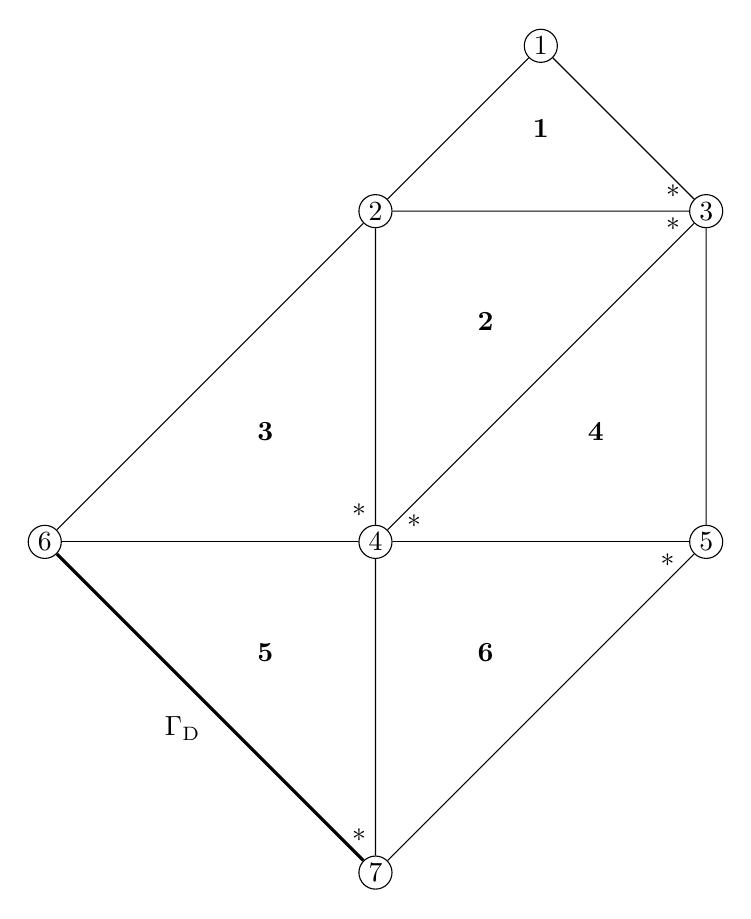
\begin{tikzpicture}[scale=0.70]
\draw[-,very thick] (-6,0) -- (0,-6);
\draw[-] (0,-6) -- (6,0) -- (6,6) -- (3,9) -- (0,6) -- (-6,0);
\draw[-] (-6,0) -- (6,0);
\draw[-] (0,-6) -- (0,6) -- (6,6) -- (0,0);
\node at (3,7.5) {\textbf{1}};
\node at (2,4) {\textbf{2}};
\node at (-2,2) {\textbf{3}};
\node at (4,2) {\textbf{4}};
\node at (-2,-2) {\textbf{5}};
\node at (2,-2) {\textbf{6}};
\draw[fill,white] (3,9)  circle (0.30); \draw (3,9) circle (0.30);
\node at (3, 9) {$1$};
\draw[fill,white] (0,6)  circle (0.30); \draw (0,6)  circle (0.30);
\node at (0, 6) {$2$};
\draw[fill,white] (6,6)  circle (0.30); \draw (6,6)  circle (0.30);
\node at  (6, 6) {$3$};
\draw[fill,white] (0,0)  circle (0.30); \draw (0,0)  circle (0.30);
\node at  (0, 0) {$4$};
\draw[fill,white] (6,0)  circle (0.30); \draw (6,0)  circle (0.30);
\node       at  (6, 0) {$5$};
\draw[fill,white] (-6,0) circle (0.30); \draw (-6,0) circle (0.30);
\node at (-6, 0) {$6$};
\draw[fill,white] (0,-6) circle (0.30); \draw (0,-6) circle (0.30);
\node       at  (0,-6) {$7$};
\node at (5.4,6.3) {*};
\node at (5.4,5.7) {*};
\node at (-0.3,0.5) {*};
\node at (0.7,0.3) {*};
\node at (-0.3,-5.4) {*};
\node at (5.3,-0.4) {*};
\node[below left] at (-3,-3) {$\Gamma_{\mathrm{D}}$};
\end{tikzpicture}
\end{center}
\end{figure}

\exercise\label{ex: 2019 exam problem}
Consider the triangulation shown in Figure~\ref{fig: 2019 exam problem}.
The global node numbers are circled and the element numbers are in bold.
The choice of the first node in each element is indicated with an asterisk,
after which the second and third follow \textbf{counterclockwise}. The
part~$\Gamma_{\mathrm{D}}$ of the boundary where a Dirichlet boundary 
condition applies is shown in a thicker line (between nodes $6$~and $7$).  Let
$\boldsymbol{f}=[f_r]$ and $\boldsymbol{A}=[a_{rs}]$ denote the global load 
vector and the global stiffness matrix, and let
$\boldsymbol{f}\brak{p}=[f\brak{p}_j]$~and 
$\boldsymbol{A}\brak{p}=[a\brak{p}_{jk}]$ denote 
the element load vector and element stiffness matrix for the $p$th element 
($1\le p\le6$).  
\begin{description}
\item{(a)} Write out the $3\times6$ connectivity matrix.
\item{(b)} Express $f_4$ as a sum over entries~$f\brak{p}_j$ of the element 
load vectors.
\item{(c)} Express $a_{22}$, $a_{35}$~and $a_{47}$ as sums over 
entries~$a\brak{p}_{jk}$ of the element matrices.
\end{description}

\begin{figure}
\caption{Triangulation for Exercise~\ref{ex: FEM triang}.}
\label{fig: FEM triang}
\begin{center}
\includegraphics[scale=1.0]{../src/chap6/ex2_triangulation-crop.pdf}
\end{center}
\end{figure}

\exercise\label{ex: FEM triang}
Consider the finite element method for a boundary-value 
problem~\eqref{eq: self-adjoint bvp 2d} using the triangulation shows in 
\cref{fig: FEM triang}.  Note that $\Gamma_{\mathrm{D}}$ consists of the bottom
and right sides of~$\Omega$ (that is, the thicker edges numbered $6$--$8$.)
\begin{description}
\item{(i)} What are $M\free$~and $M\fix$, the numbers of free and fixed nodes?
\item{(ii)} What is $Q_{\mathrm{N}}$, the number of edges 
along~$\Gamma_{\mathrm{N}}$?
\item{(iii)} Write down the triangle connectivity 
matrix~$\boldsymbol{T}^{\mathcal{K}}$.
\item{(iv)} Write down the edge connectivity 
matrix~$\boldsymbol{T}^{\mathcal{E}}$.
\item{(v)} What are the dimensions of the global load 
vector~$\boldsymbol{f}=[f_r]$, the global stiffness 
matrix~$\boldsymbol{A}=[a_{rs}]$ and the global Neumann 
vector~$\boldsymbol{g}_{\mathrm{N}}=[g_{\mathrm{N},r}]$?
\item{(vi)} Express each $f_r$ as a sum of entries~$f\brak{p}_i$ from the 
element load vectors $\boldsymbol{f}\brak{1}$, $\boldsymbol{f}\brak{2}$, \dots,
$\boldsymbol{f}\brak{10}$.
\item{(vii)} Express each nonzero~$a_{rs}$ as a sum of entries~$a\brak{p}_{ij}$
from the element stiffness matrices $\boldsymbol{A}\brak{1}$, 
$\boldsymbol{A}\brak{2}$, \dots, $\boldsymbol{A}\brak{10}$.  (From symmetry, it 
suffices to list the cases with $r\le s$.)
\item{(viii)} Express each $g_{\mathrm{N},r}$ as a sum of 
entries~$g^{[q]}_{\mathrm{N},r}$ of the edge Neumann vectors 
$\boldsymbol{g}^{[1]}_{\mathrm{N}}$, $\boldsymbol{g}^{[2]}_{\mathrm{N}}$, \dots
$\boldsymbol{g}^{[5]}_{\mathrm{N}}$.
\end{description}

\end{Exercises}
